 \chapter{ Algoritmos de extracción y descripción de características}
 
Las características de los objetos son cualidades que nos servirán para identificarlos dentro de una imagen donde pueden existir objetos similares. Para poder discernir de los objetos que estén en la imagen nos basamos en las características encontradas, que serán encapsuladas en un descriptor. Un descriptor de un objeto es la representación, de una manera reducida, de todas las características que se pueden obtener de toda la información del objeto, esto facilitara la comparación entre los diferentes objetos que existan en una imagen.
Para extraer las características existen diferentes formas, dependerá de que algoritmo se utilice. Y para generar un descriptor, es la misma situación, dependerá del algoritmo. En este capítulo se explicarán dos algoritmos para extraer características y generar su descriptor.   

\section{Scale-Invariant Feature Transform SIFT}
	El algoritmo de SIFT, propuesto por Lowe en \cite{Lowe2004},  provee un método robusto para la extracción de puntos característicos que se utilizan para generar el descriptor. Los puntos que se encuentran son invariantes a diferentes transformaciones como traslación, escalamiento y rotación. Han mostrado tener un amplio rango de tolerancia a transformaciones afines, adición de ruido y cambios de iluminación. A continuación se describirán los pasos del algoritmo para la generación del conjunto de puntos característicos:
\pagebreak
	\subsection{Detección de puntos extremos en el Espacio-Escala} \hfill \\
		Se realiza una búsqueda en las imágenes en todo el espacio escala, para localizar puntos extremos se debe identificar su ubicación y escala, para volver a encontrarlos no importando la vista o tamaño del mismo objeto.\\
		El espacio escala es un conjunto de imágenes, que se forman a partir de suavizar la imagen original a diferentes niveles de detalles, los cuales son definidos por un parámetro $\sigma$. Está representado por la función $L(x,y;\sigma)$ la cual se forma por la convolución con $G(x,y;\sigma)$ y la imagen original $I(x,y)$:
		$$L(x,y;\sigma) = G(x,y;\sigma) * I(x,y)$$
		Donde $*$ es el operador convolución en $x$ y $y$, y
		$$ G(x,y;\sigma) = \frac{1}{2\pi\sigma^2}e^{\frac{-(x^2+y^2)}{2\sigma^2}}$$
		\begin{figure}[h]
			\centering
				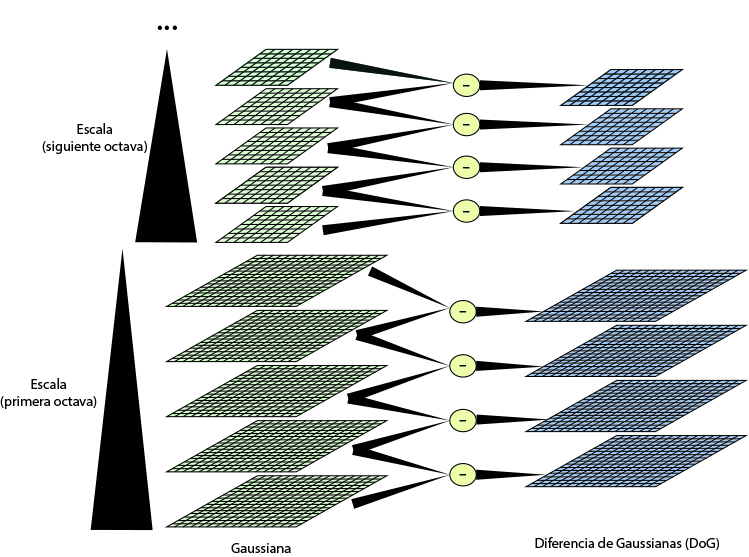
\includegraphics[scale=0.5]{img/spaceScale.jpg}
			\caption{Espacio Escala de Diferencia de Gaussianas}
		\end{figure}		
		Para la detección de puntos extremos estables se aplicará el espacio escala, usando diferencias de gaussianas convolucionadas con una imagen, en lugar de solo un filtro gaussiano, $D(x,y;\sigma)$  que podremos calcular por la diferencia de dos escalas cercanas separadas por un factor $k$ multiplicativo:
		$$D(x,y;\sigma) = (G(x,y;k\sigma) - G(x,y;\sigma)) * I(x,y)$$ $$= L(x,y;k\sigma) - L(x,y;\sigma)$$
		La diferencia de gaussianas es una aproximación muy cercana a el laplaciano de gaussiana (LoG) normalizado en escala, $\sigma^2 \nabla^2 G$. La normalización hecha con el factor $\sigma^2$ es necesaria para poder asegurar que el algoritmo sera invariante a los cambios en tamaño. La relación entre D y $\sigma^2 \nabla^2 G$ es una ecuación en derivadas parciales:
		$$\frac{\partial G}{\partial \sigma} = \sigma \nabla^2 G$$
		Podemos ver que $\nabla^2 G$ se puede calcular con una aproximación de diferencias finitas de  $\frac{\partial G}{\partial \sigma}$, usando diferencias de escalas próximas de $k\sigma$ y $\sigma$:
		$$ \sigma \nabla^2 G = \frac{ \partial G}{\partial \sigma} \approx  \frac{G(x , y , k \sigma) - G( x , y, k \sigma)}{k \sigma - \sigma}$$
		y por lo tanto,
		$$ G(x , y , k \sigma) - G( x , y, k \sigma) \approx (k - 1)\sigma^2 \nabla^2 G $$
		En la figura 2-1 se puede ver la construcción de $D(x,y,\sigma)$. La imagen inicial se convoluciona con diferentes mascaras gaussianas, para producir imágenes separadas por un factor constante $k$ en el espacio escala. Se divide cada octava del espacio escala entre un numero entero, s, de intervalos entonces $k= 2^\frac{1}{s}$. Se producen $s+3$  imágenes emborronadas en la pila, por octava.
		\begin{figure}[h]
			\centering
				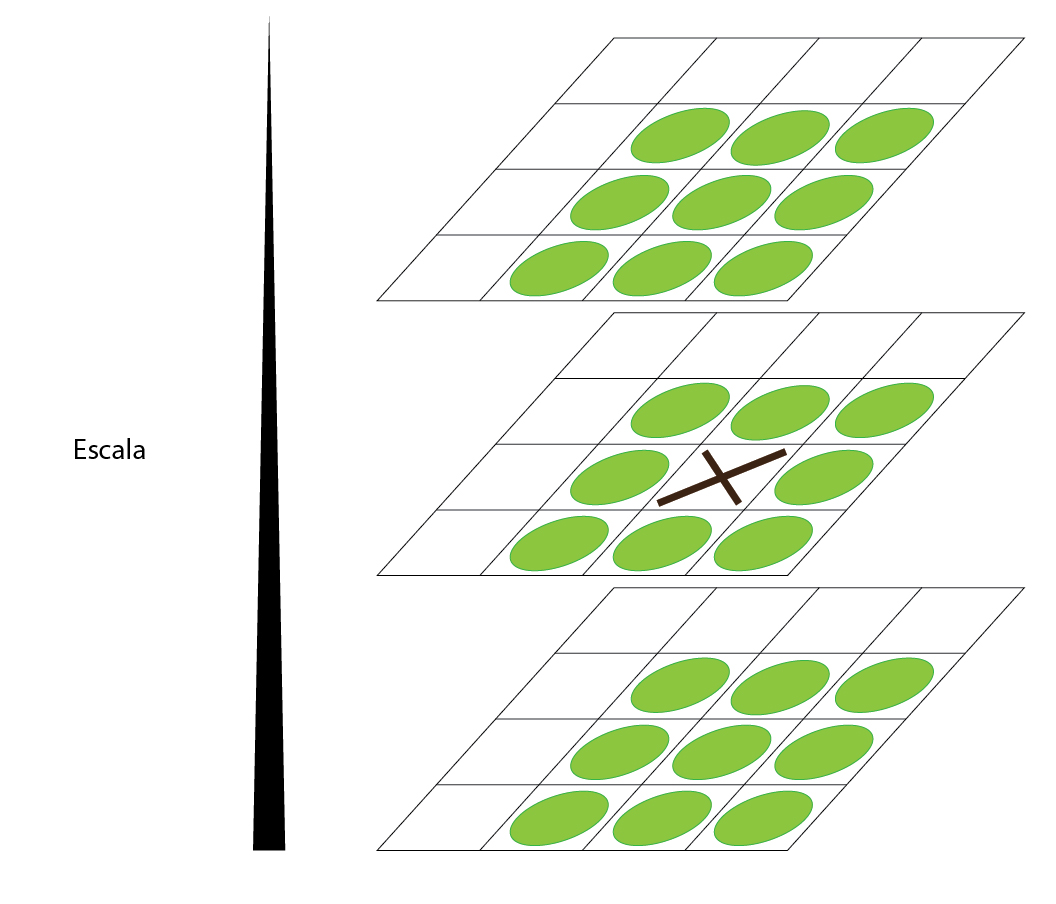
\includegraphics[scale=0.15]{img/EscalaPuntosExtremos.jpg}
			\caption{Espacio Escala de Diferencia de Gaussianas}
		\end{figure}
		Para extraer las ubicaciones máximas y mínimas (puntos extremos) en $D(x,y,\sigma)$, cada punto es comparado con sus ocho vecinos en la misma imagen y con sus otros dieciocho vecinos de escala, nueve en la imagen de arriba y nueve en la imagen de abajo (Figura 2-2). Solo se selecciona el punto si es el más grande o el más pequeño de entre todos sus vecinos.
	
	
	
	
	\subsection{Localización de puntos característicos} \hfill \\  %%Poner una imagen de los puntos obtenidos si hacer los diferentes filtrop para los outliers
		Una vez que se seleccionaron los puntos extremos, se aplica una medida de estabilidad sobre todos para descartar aquellos que no sean adecuados, para obtener puntos  característicos de forma precisa. Existen dos casos donde los puntos extremos anteriormente seleccionados tendrían que ser eliminados:
	\begin{enumerate}
		\item El punto tiene un contraste muy bajo.
		\item El punto está localizado sobre un borde.
	\end{enumerate}			
	Para eliminar los puntos del caso uno, primero debemos obtener la serie de Taylor del espacio escala $D(x,y,\sigma)$:
		$$D(X)=D +\frac{\partial D}{\partial X}^T X+ \frac{1}{2} X^T\frac{\partial^2 D}{\partial X^2} X $$
		donde la $D$ y su derivada son evaluadas en el punto $X = (x,y,\sigma)^T$ cuando se deriva esta función respecto a $X$ y se iguala a cero podemos encontrar los valores extremos: 
	    $$ \hat{X} = - \frac{\partial^2 D}{\partial X^2}^{-1}\frac{\partial D}{\partial X}$$
	 	La función que evaluara al punto extremo sera, $D(\hat{X})$, la cual rechazara al punto si es de muy bajo contraste, la cual se obtiene de sustituir $\hat{X}$ en $D(X)$:
	 	$$D(\hat{X})=D + \frac{1}{2} \frac{\partial D}{\partial X}^T \hat{X} $$ 	 
	 	En el trabajo de Lowe \cite{Lowe2004}, se  puede ver que encontraron experimentalmente que cualquier valor extremo menor de 0.03 es descartado:
	 	$$ |D(\hat{X})|< 0.03$$ 	 
	 	Para el segundo caso, se utiliza una matriz Hessiana de $2\times2$, $H$, la cual se calcula en la escala y lugar del punto extremo:
		$$ 
		H
		=
		\begin{bmatrix}
			D_{xx} & D_{xy}\\
    		D_{xy} & D_{yy}
		\end{bmatrix}		 	
		$$	
		Los valores propios de H son proporcionales a las curvaturas de D. Se toma prestado el criterio que se usa para la detección de esquinas usando el algoritmo de Harris \cite{Harris1988}, se puede evitar el calculo de los valores propios ya que solo nos interesa su relación. Sea $\alpha$ el valor propio de mayor magnitud y $\beta$ el de menor. Entonces podemos calcular la suma de los valores propios de la diagonal de $H$ y su producto por medio del determinante:
		$$Tr(H) = D_{xx} + D_{yy} = \alpha+\beta,$$ $$Det(H) = D_{xx}D_{yy}-(D_{xy})^2= \alpha\beta$$
		Sea $r$ la razón de la magnitud que existe entre $\alpha$ y $\beta$, $\alpha = r\beta$. Entonces:
		$$\frac{Tr(H)^2}{Det(H)}= \frac{(\alpha+\beta)^2}{\alpha\beta}= \frac{(r\beta+\beta)^2}{r\beta^2}= \frac{(r+1)^2}{r}$$
		el cual solo depende de la razón de los valores propios y no de los valores individuales. El valor de $\frac{(r+1)^2}{r}$, es mas pequeño cuando los valores propios son iguales e incrementa con $r$.Entonces para cerciorar que la razón de las curvas principales es menor que cierto umbral, $r$, solo se necesita:
		$$\frac{Tr(H)^2}{Det(H)} < \frac{(r+1)^2}{r}$$
		En la publicación de Lowe \cite{Lowe2004} se encontró un valor experimental para $r=10$, que elimina los puntos extremos que tengan la razón entre las dos curvas mayor que 10.
	
	
	\subsection{Asignación de orientación} \hfill \\
		Por medio de la asignación de una orientación a cada punto característico, basado en propiedades locales de la imagen, el descriptor que encontremos sera invariante a la rotación. La ubicación en el espacio escala del punto característico, es usada para seleccionar la imagen suavizada por una mascara gaussiana, $L$, esto provocara que sea invariante a la escala. Para cada muestra de la imagen, $L(x,y)$, la magnitud del gradiente, $m(x,y)$, y la orientación ,$\theta(x,y)$, son precalculadas por medio de diferencias de gaussianas:
  		$$m(x,y) = \sqrt{ (L(x+1,y)-L(x-1,y))^2 + (L(x,y+1)-L(x,y-1))^2 }$$		
		$$\theta(x,y) =  \tan^{-1} \left(\frac{L(x,y+1)-L(x,y-1)}{L(x+1,y)-L(x-1,y)}\right)$$
		Se formara un histograma de orientaciones que tendrá la orientación de los gradientes calculados en una región, al rededor del punto característico, el tamaño de esta muestra dependerá de la ubicación en el espacio escala en la que se encuentre el punto característico. El histograma de orientaciones tendrá 36 divisiones cubriendo los 360 grados.
		\begin{figure}[t]
			\centering
				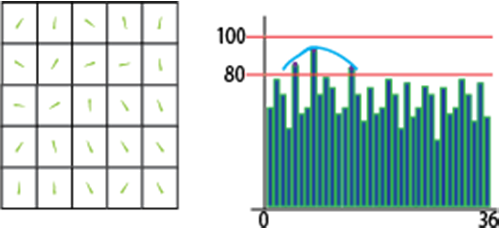
\includegraphics[scale=0.5]{img/HistoOrientacion.png}
			\caption{Histograma de Orientación TEMPORAL}
		\end{figure}
		Para cada muestra agregada se ponderada por la magnitud de su gradiente y por una mascara circular gaussiana ponderada con $\sigma$, que es $1.5$ veces que de la ubicación del espacio escala donde reside el punto característico.
		Los picos en el histograma de orientación corresponden a las direcciones dominantes de los gradientes locales. Se encuentra el pico mas grande y cualquier otro pico que se encuentre en el rango de $100\% - 80\%$, del pico más grande, se utiliza para hacer que el punto característico tenga una orientación. Para ubicaciones con varios picos de magnitudes similares, se generaran puntos característicos con la misma ubicación y escala pero con diferentes orientaciones. Solo el $15\%$ de los puntos se les asignan múltiples orientaciones, pero aun así esto contribuye mucho al momento de emparejar. Finalmente se obtiene una parábola usando como puntos tres picos cercanos entre si, para interpolar la posición del pico con mas precisión.  
	
	
	\subsection{Descriptor de puntos característicos} \hfill \\
	Hasta este momento tenemos una colección de puntos característicos, los cuales están formados por una ubicación, una escala y una orientación. Ahora debemos formar un descriptor que sea lo suficientemente distintivo. Para esto tenemos que tomar una muestra de la imagen, al rededor del punto característico de $16\times16$ pixeles y se dividirá en una región de $4 \times 4$. Se generará un histograma de orientación de los gradientes de cada región, a diferencia del histograma de orientación explicado anteriormente, el histograma solo tiene 8 divisiones con las cuales se cubrirán los 360 grados, igualmente se usara una ponderación gaussiana para la asignación de la magnitud al histograma.
		\begin{figure}[t]
			\centering
				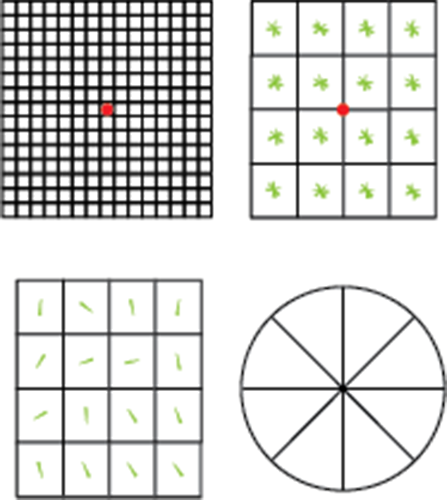
\includegraphics[scale=0.5]{img/Descriptor.png}
			\caption{Descriptor TEMPORAL}
		\end{figure}
	Al final el descriptor de cada punto característico estará formado por un vector, que tiene las ocho orientaciones de los $4\times4$ histogramas. Por lo tanto el tamaño del vector sera de $4\times4\times8 = 128$ elementos. 
 
 
 




%\section{}



